% arara: pdflatex: { shell: true }
% arara: biber
% arara: pdflatex: { shell: true }
% arara: pdflatex: { shell: true }
\documentclass[12pt]{report}

\usepackage{graphicx, color}
\usepackage[utf8]{inputenc}
\usepackage[english]{babel}
\usepackage[a4paper,margin=2cm]{geometry}
\usepackage[backend=biber]{biblatex}
\usepackage{hyperref}
\usepackage{csquotes}
\usepackage{pgfplots}
\usepackage{pgfplotstable}
\usepackage{tikz}
\usepackage{mathtools}
\usepackage{amsmath}
\usepackage{amsfonts}

%\usepgfplotslibrary{external}
\pgfplotsset{compat = newest}
%\tikzexternalize[prefix=tikz/]

\addbibresource{bibentries.bib}

\newcommand{\red}[1]{{\color{red}{#1}}}


\begin{document}

    \begin{titlepage}


        \newcommand{\HRule}{\rule{\linewidth}{0.5mm}} % Defines a new command for the horizontal lines, change thickness here

        \center % Center everything on the page


%----------------------------------------------------------------------------------------

%	HEADING SECTIONS

%----------------------------------------------------------------------------------------


        \textsc{\Large MSc Artificial Intelligence}\\[0.2cm]

        \textsc{\Large Master Thesis}\\[0.5cm]


%----------------------------------------------------------------------------------------

%	TITLE SECTION

%----------------------------------------------------------------------------------------



        \HRule \\[0.4cm]

        { \huge \bfseries \red{Your Title Here}}\\[0.4cm] % Title of your document

        \HRule \\[0.5cm]


%----------------------------------------------------------------------------------------

%	AUTHOR SECTION

%----------------------------------------------------------------------------------------



        by\\[0.2cm]

        \textsc{\Large \red{Your Name}}\\[0.2cm] %you name

        \red{student number}\\[1cm]


%----------------------------------------------------------------------------------------

%	DATE SECTION

%----------------------------------------------------------------------------------------



        {\Large \today}\\[1cm] % Date, change the \today to a set date if you want to be precise



        \red{Number of Credits}\\ %

        \red{Period in which the research was carried out}\\[1cm]%


%----------------------------------------------------------------------------------------

%	COMMITTEE SECTION

%----------------------------------------------------------------------------------------

        \begin{minipage}[t]{0.4\textwidth}

            \begin{flushleft}
                \large

                \emph{Supervisor:} \\

                \red{Dr A \textsc{Person} }% Supervisor's Name

            \end{flushleft}

        \end{minipage}

        ~

        \begin{minipage}[t]{0.4\textwidth}

            \begin{flushright}
                \large

                \emph{Examiner:} \\

                \red{Dr A  \textsc{Person}}\\

                \vspace{0.5cm}

                \emph{Second reader:} \\

                \red{Dr A  \textsc{Person}}\\

            \end{flushright}

        \end{minipage}\\[2cm]


%----------------------------------------------------------------------------------------

%	LOGO SECTION

%----------------------------------------------------------------------------------------




        
\includegraphics[width=10cm]{uvalogo_regular_p_nl.eps}


%----------------------------------------------------------------------------------------



        \vfill % Fill the rest of the page with whitespace

    \end{titlepage}

    \pagenumbering{roman}

    \tableofcontents

    \begin{abstract}
        \red{Provide a short overview and description of your thesis here.}
    \end{abstract}

    \pagenumbering{arabic}


    \chapter{Introduction}

    \red{This document provides an empty template for your thesis. Please keep the following things in mind when writing your thesis:
        \begin{itemize}
            \item The chapter organization of this template is a generic suggestion, please customize to your needs and vision.
            \item The guideline is to have a 40 page upper limit for the thesis, with additional optional pages for appendices if needed, for example to provide additional experimental results or mathematical details. Most theses do not end up with an appendix.
            \item For references, you are free to choose your own style. A standard style is included in this template, for example~\cite{lecun2015deep}.
            \item The official website of the thesis AI (https://student.uva.nl/ai/content/az/master-thesis-ai/master-thesis-ai-2020.html) contains all information regarding the procedures and details of the thesis process.
        \end{itemize}}


    \chapter{Related work}


    \section{Pass-through trick}
    BinnaryConnect: Use the passthrough trick to learn binary (-1 or 1) neural networks~\cite{courbariauxBinaryConnectTrainingDeep2016, hubaraBinarizedNeuralNetworks}

    Ternary weight networks ~\cite{liTernaryWeightNetworks2022, zhuTrainedTernaryQuantization2017}

    Piggyback: Earliest paper I found (2018) which does the submasking method with the ‘pass-through’ trick. They actually use it for finetuning models like us.~\cite{mallyaPiggybackAdaptingSingle2018}

    NASpaper: NAS paper which, independently from the Piggyback paper, used similar tricks for performing neural architecture
    search~\cite{wortsmanDiscoveringNeuralWirings2019a}

    Ramanujan et al: Inspired by the NASPaper, they rediscovered the Piggyback method except applied it to training models from scratch and they also control the sparsity (piggy uses a threshold method).~\cite{ramanujanWhatHiddenRandomly2020}

    Movement Pruning: They prune models by applying ramanujan’s submasking and the Piggyback method in tandem with training the weights of the neural network (NLP). They use the term ‘hard’ movement pruning to refer to Ramanujan’s method (top k\%) and ‘soft’ pruning to refer to the Piggyback method (prune if score higher than threshold). They additionally enhance the pruning by adding a knowledge distillation loss as well.~\cite{sanhMovementPruningAdaptive}

    Block Movement Pruning: They do movement pruning with also distillation but by grouping ‘blocks’ of weights together into the same masking unit (so all weights in the block share a mask). Seems to work quite well.~\cite{lagunasBlockPruningFaster2021}

    Supsup: Very cool use of the submasking method: They make a random network learn thousands of different tasks, each task with it’s own supermask. They base it primarily on Ramanujan et al but also mention Piggyback and argue that their method is superior.~\cite{wortsmanSupermasksSuperposition}

    Packnet: Paper doing iterative pruning and retraining to teach a network new tasks ~\cite{mallyaPackNetAddingMultiple2018}

    Very recent paper that explores the best ways to fine-tune several models including resnets, vits, and convnexts.
    Their significant contribution is to freeze the the transformer embeddings in order to get the same performance with SGD as you can get with Adam. They get the highest CLIP-finentuned cifar-10 performance I have seen so far so it is a very good baseline to compare accuracies against~\cite{kumarHowFineTuneVision2022}



    \section{Self-supervision}

    Momentum contrast uses an embedding queue in combination with distinct key and query embedders such that the query embedder is trained through backpropagation on the current mini-batch (contrasted against all key embeddings in the queue) and the key embedder is updated by slowly adding the query embedder's parameters to it. Importantly, batch normalization needs to be disabled or shuffled.~\cite{heMomentumContrastUnsupervised2020}

    Dino is similar to momentum contrast except rather than using embeddings and a queue it just applies a cross-entropy loss between the teacher (key embedder) and student (query embedder) logits. It however needs to apply 'centering' and 'sharpening' to avoid collapse.~\cite{caronEmergingPropertiesSelfSupervised2021a}

    SLIP is an improvement over CLIP which also makes use of self-supervision for pretraining.~\cite{muSLIPSelfsupervisionMeets2021}

    Pretraining using self-supervision, then pre-training again using self-supervision but on the target dataset, and finally supervised-finetuning of a classifier head works well in NLP~\cite{gururanganDonStopPretraining2020, howardUniversalLanguageModel2018}

    \section{Ensembling}
    Ensembles of smaller models appear to outperform larger models.~\cite{kondratyukWhenEnsemblingSmaller2020}

    \chapter{Method}

    \section{SGD is an EMA}

%    \[
%%        \label{eq:ema}
%        \theta_{t+1} &= \gamma \theta_{t+1\|\theta_t,g_t} + (1-\gamma) \theta_{t}\\
%        \theta_{t+1} &=
%    \]
    \begin{align}
        \label{eq:ema}
        \theta_{t+1} &= \theta_{t} - g_{t+1}\gamma_{t+1}\\
        \theta_{t+1} &= \theta_{t} - g_{t+1}\gamma_{t+1} + \theta_t\gamma_{t+1} - \theta_t\gamma_{t+1}\\
        \theta_{t+1} &= \theta_{t} + (\theta_t - g_{t+1})\gamma_{t+1} - \theta_t\gamma_{t+1}\\
        \theta_{t+1} &= (\theta_t - g_{t+1})\gamma_{t+1} + \theta_t(1 - \gamma_{t+1})\\
        \theta_{t+1} &= \theta_{t+1\|\theta_t,g_{t+1}} \gamma_{t+1} + \theta_{t}(1-\gamma_{t+1})
    \end{align}


    \section{Translation invariance of threshold and score initialization}

    \begin{align}
%        \label{eq:threshold}
        m_i^t &= [\theta_i^t > k]
    \end{align}

    where $k$ is the threshold

    \begin{align}
        \theta_i^{t} &= \theta_i^0 - \sum_{\hat t=0}^{t-1} \gamma^{\hat t} g_{i}(\mathcal{M}^{\hat t}, \mathcal{B}^{\hat t})
    \end{align}

    where $g_{i}(\mathcal{M}^{\hat t}, \mathcal{B}^{\hat t})$ is the gradient of the $i$'th weight given the mask $\mathcal{M}^{\hat t}$ and batch $\mathcal{B}^{\hat t}$ (including momentum if enabled)

    \begin{align}
        m_i^0 &= [\theta_i^0 > k] &= [\theta_i^0 + a > k + a] \\
        m_i^{t} &= [\theta_i^0 - \sum_{\hat t=0}^{t-1} \gamma^{\hat t} g_{i}(\mathcal{M}^{\hat t}, \mathcal{B}^{\hat t}) > k] &= [\theta_i^0 + a - \sum_{\hat t=0}^{t-1} \gamma^{\hat t} g_{i}(\mathcal{M}^{\hat t}, \mathcal{B}^{\hat t}) > k + a]\label{eq:recur}
    \end{align}

    For the base case we then have that replacing $\theta_i^0$ with $\theta_i^0 + a$ and $k$ with $k+a$ will not change $m_i^0$ for any $i$, which means the network mask $\mathcal{M}^0$ is also invariant to this change.
    Consequently, $m_i^1$ is also invariant to this change because of eq.~\ref{eq:recur} and because the gradient $g_i(\mathcal{M}^0, \mathcal{B}^0)$ does not change. The same reasoning can be applied recursively to $m_i^2$ and so on. Thus, by induction, translating the initial score and threshold by the same amount will not change any of the network masks during training (under simple sgd without weight decay).

    \section{Scale invariance of learning rate and score initialization}

    Equation for sgd with weight decay:

    \begin{align}
        \theta_i^t &= \theta_i^{t-1} - \gamma^t \left( g_i(\mathcal{M}^{t-1}, \mathcal{B}^{t-1}) + \lambda \theta_i^{t-1} \right)
    \end{align}

    Say we replace $\gamma^t$ with $\gamma^t \alpha$, $\theta_i^{t-1}$ with $\theta_i^{t-1} \alpha$ and $\lambda$ with $\frac{\lambda}{\alpha}$ for some $\alpha \in \mathbb{R}^+$, then we get:

    \begin{align}
        \alpha\theta_i^{t-1} - \alpha\gamma^t \left( g_i(\mathcal{M}^{t-1}, \mathcal{B}^{t-1}) + \frac{\lambda}{\alpha} \alpha\theta_i^{t-1} \right) &= \alpha \left(\theta_i^{t-1} - \gamma^t \left( g_i(\mathcal{M}^{t-1}, \mathcal{B}^{t-1}) + \lambda \theta_i^{t-1} \right)\right)\\
        &= \alpha\theta_i^{t}\label{eq:krrrt}
    \end{align}

    Similarly to the previous proof, the initial masks $m_i^0 = [\theta_i^0 > 0]$ are invariant to the scale change $m_i^0 = [\alpha\theta_i^0 > 0]$, so the replacement of $\theta_i^0$ with $\alpha\theta_i^0$, combined with the other replacements, does not change the gradient $g_i(\mathcal{M}^0, \mathcal{B}^0)$.  Combined with eq \ref{eq:krrrt}, this means that the updated parameter after the first SGD step is only different in scale when compared to what it would have been without the scale change ($=\alpha\theta_i^t$). Apply this reasoning recursively and it can be seen through induction that the network masks will be the same during training as for the original learning rate, score initialization and weight decay.

    Note that the conclusion still holds when momentum is enabled
    \chapter{Experiments}

    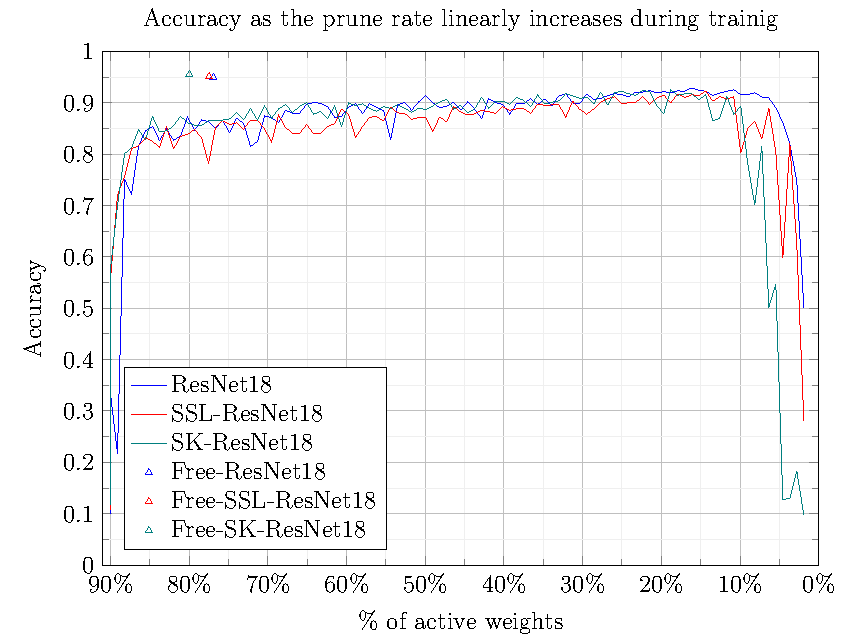
\includegraphics[width=1.0\textwidth]{plots/variant_sparsity.pdf}

%% https://latexdraw.com/plot-a-function-and-data-in-latex/
%    \pgfplotstableread{plots/plot_data/variant_sparsity.csv}{\table}
%
%    \begin{tikzpicture}
%        \begin{axis}[
%            title={Accuracy as the prune rate linearly increases during trainig},
%            xlabel={\% of active weights},
%            ylabel={Accuracy},
%            x dir=reverse,
%            xmin = 0, xmax = 90,
%            ymin = 0, ymax = 1,
%            xtick distance = 10,
%            ytick distance = 0.1,
%            grid = both,
%            minor tick num = 1,
%            major grid style = {lightgray},
%            minor grid style = {lightgray!25},
%            width = \textwidth,
%            height = 0.75\textwidth,
%            legend cell align = {left},
%            legend pos = south west
%        ]
%
%            \addplot[blue] table [x expr= \thisrow{sparsity}*100, y = {resnet18}] {\table};
%
%            \addplot[red] table [x expr= \thisrow{sparsity}*100, y = {ssl_resnet18}] {\table};
%
%            \addplot[teal] table [x expr= \thisrow{sparsity}*100, y = {skresnet18}] {\table};
%
%            \legend{
%                ResNet18,
%                SSL-ResNet18,
%                SK-ResNet18
%            }
%
%        \end{axis}
%
%    \end{tikzpicture}


    \chapter{Conclusions}


    \appendix


    \chapter{Optional appendix}

    \printbibliography

\end{document}

